\documentclass[sigconf,nonacm]{acmart} % 加入 nonacm 选项

\settopmatter{printacmref=false} % 移除 ACM reference 格式
\setcopyright{none}             % 移除版权/权限声明
\renewcommand\footnotetextcopyrightpermission[1]{} % 清除底部的会议信息

\usepackage{graphicx}
\usepackage{algorithm}
\usepackage{algorithmic}
\usepackage{amsmath}
\usepackage{cleveref}
\usepackage{booktabs} % 添加以支持高质量表格

\title{Comparative Analysis of Recommendation System Algorithms}

\author{Jiepei Chen}
\affiliation{
  \institution{City University of HongKong (Dongguan)}
}
\email{72405876@cityu-dg.edu.cn}

\author{Hao Yang}
\affiliation{
  \institution{City University of HongKong (Dongguan)}
}
\email{72403219@cityu-dg.edu.cn}

\author{Lu Peng}
\affiliation{
  \institution{City University of HongKong (Dongguan)}
}
\email{72401459@cityu-dg.edu.cn}

\author{Xuanhao Yan}
\affiliation{
  \institution{City University of HongKong (Dongguan)}
}
\email{72405380@cityu-dg.edu.cn}

\author{Zexuan He}
\affiliation{
  \institution{City University of HongKong (Dongguan)}
}
\email{72403000@cityu-dg.edu.cn}
 
\begin{document}


\fancyhead{} % 清除页眉

\begin{abstract}

This study presents a systematic evaluation of diverse recommendation algorithms across three benchmark datasets: MovieLens, Last.FM, and Yelp. We investigate traditional collaborative filtering approaches (user-based, item-based), matrix factorization techniques (SVD), and advanced graph neural network methods (LightGCN, NGCF). Additionally, we also employ content-based methods for the MovieLens dataset and friend-based approaches for the Last.FM dataset, tailored to the distinct characteristics of each dataset. Through rigorous empirical comparison using ranking-based metrics (HR@K, NDCG@K, MRR@K), we identify the strengths and limitations of each approach under varying data conditions, including sparsity levels and cold-start scenarios. Our findings reveal that while GNN-based methods generally outperform traditional approaches on denser datasets, collaborative filtering techniques maintain competitive performance in specific contexts, particularly with sparse interaction data. This comparative analysis provides practical insights for algorithm selection based on dataset characteristics and application requirements.  

Source code for implementation is available at \url{https://github.com/jasper7c/CS5481-RecommenderSystem}. 
\end{abstract}

\maketitle

\section{Introduction}
Personalized recommendation systems are essential tools to handle information overload, facilitating content filtering based on individual user interests and preferences. These systems significantly enhance user experience by predicting items of potential interest \cite{ricci2011introduction}. With the explosive growth of online information, recommender systems have become indispensable components in various domains including e-commerce, entertainment, social media, and information retrieval \cite{adomavicius2005toward}.

The field of recommender systems has evolved through several phases. Initially, content-based filtering methods analyzed item features to recommend similar items to users \cite{pazzani2007content}. However, these approaches struggled with the "overspecialization" problem, limiting discovery of diverse items. Traditionally, collaborative filtering (CF) methods, particularly user-based and item-based algorithms \cite{sarwar2001item}, have dominated applied settings due to simplicity and interpretability. Yet, these methods face challenges with data sparsity, cold-start problems, and scalability issues \cite{su2009survey}.

Matrix factorization techniques such as Singular Value Decomposition (SVD) efficiently capture latent user and item characteristics through dimensionality reduction, thus addressing data sparsity challenges \cite{koren2009matrix}. The Netflix Prize competition significantly advanced these methods, demonstrating their effectiveness in real-world recommendation tasks \cite{bell2007lessons}.

Recently, Graph Neural Networks (GNNs) have emerged, capturing complex user-item interactions via graph-structured data representations. Methods like LightGCN \cite{he2020lightgcn} and NGCF \cite{wang2019neural} overcome limitations inherent in traditional models by effectively leveraging neighborhood structural information. These approaches excel particularly in capturing higher-order connectivity patterns that are difficult to model with conventional matrix-based methods \cite{wu2022graph}.

For our empirical analysis, we selected three widely-used benchmark datasets with distinct characteristics:  
\begin{itemize}  
    \item \textbf{MovieLens (1M)}: Contains 1,000,209 ratings from 6,040 users on approximately 3,900 movies, representing a medium-density entertainment domain \cite{movielens}.  
    \item \textbf{Last.FM}: Comprises music listening preferences of 1,892 users across 92,800 artists, characterized by high sparsity and diverse interaction patterns \cite{lastfm}.  
    \item \textbf{Yelp}: A large-scale dataset containing 6,990,280 reviews across 11 metropolitan areas for 150,346 businesses, featuring rich contextual information and geographic diversity \cite{yelp}.  
\end{itemize}  

This study makes several contributions:  
\begin{itemize}  
    \item A comprehensive cross-method evaluation using consistent preprocessing and evaluation protocols, enabling direct performance comparisons across algorithmic approaches  
    \item Analysis of algorithm performance under varying data conditions, including different sparsity levels and interaction patterns  
    \item Practical guidelines for algorithm selection based on dataset characteristics and application requirements  
    \item Reproducible implementation of recommendation algorithms with optimized hyperparameter configurations  
\end{itemize}  


\section{Related Work}
\subsection{Collaborative Filtering}
CF approaches generally rely on computing similarity between users or items to generate recommendations. User-based CF measures user-user similarity to predict unknown user preferences. Item-based CF, conversely, calculates item-item similarity for recommendation \cite{sarwar2001item}.

The prediction of rating $r_{ui}$ for user $u$ and item $i$ in user-based CF typically follows:
\begin{equation}
r_{ui} = \frac{\sum_{v \in N(u)} sim(u,v) \cdot r_{vi}}{\sum_{v \in N(u)}|sim(u,v)|}
\label{eq:userbased}
\end{equation}
where $N(u)$ denotes the neighborhood of user $u$, and $sim(u,v)$ refers to similarity between users.

Similarly, item-based CF predicts ratings as:
\begin{equation}
r_{ui} = \frac{\sum_{j \in N(i)} sim(i,j) \cdot r_{uj}}{\sum_{j \in N(i)}|sim(i,j)|}
\label{eq:itembased}
\end{equation}
where $N(i)$ represents similar items to item $i$.

Common similarity metrics include Pearson correlation coefficient:
\begin{equation}
sim_{pearson}(u,v) = \frac{\sum_{i \in I_{uv}}(r_{ui} - \bar{r}_u)(r_{vi} - \bar{r}_v)}{\sqrt{\sum_{i \in I_{uv}}(r_{ui} - \bar{r}_u)^2}\sqrt{\sum_{i \in I_{uv}}(r_{vi} - \bar{r}_v)^2}}
\label{eq:pearson}
\end{equation}
and cosine similarity:
\begin{equation}
sim_{cosine}(u,v) = \frac{\sum_{i \in I_{uv}}r_{ui} \cdot r_{vi}}{\sqrt{\sum_{i \in I_{uv}}r_{ui}^2}\sqrt{\sum_{i \in I_{uv}}r_{vi}^2}}
\label{eq:cosine}
\end{equation}
where $I_{uv}$ represents items rated by both users $u$ and $v$.

\subsection{Matrix Factorization: SVD}
Matrix factorization methods model user-item interactions into latent factor spaces. Singular Value Decomposition (SVD) factorizes the interaction matrix $R \in \mathbb{R}^{m \times n}$ into the product of three matrices:
\begin{equation}
R = U \Sigma V^T
\label{eq:svd}
\end{equation}
where $U \in \mathbb{R}^{m \times k}$ and $V \in \mathbb{R}^{n \times k}$ are orthogonal matrices, capturing latent user and item features respectively, and $\Sigma \in \mathbb{R}^{k \times k}$ is a diagonal matrix of singular values.

In practice, a regularized version known as Regularized SVD or probabilistic matrix factorization is often used, modeled as:
\begin{equation}
\  min_{p,q} \frac{1} {2} \sum_{(u,i) \in \Omega} (r_{ui} - p_u^T q_i)^2 + \lambda (||p_u||^2 + ||q_i||^2)
\label{eq:regsvd}
\end{equation}
where $p_u$ and $q_i$ are latent vectors for user $u$ and item $i$, $\Omega$ denotes observed ratings, and $\lambda$ controls regularization.

\subsection{Graph Neural Networks}
Graph Neural Networks model the recommendation problem as a bipartite graph where users and items are nodes, and interactions form edges.

\subsubsection{Neural Graph Collaborative Filtering (NGCF)} 
NGCF explicitly incorporates higher-order connectivities between users and items by propagating embeddings through multiple graph convolutional layers \cite{wang2019neural}.
In the initial step, each user and item is associated with an ID embedding. Let $\mathbf{e}_u^{(0)}$ denote the ID embedding of user $u$ and $\mathbf{e}_i^{(0)}$ denote the ID embedding of item $i$. Then NGCF leverages the user-item interaction graph to propagate embeddings as:  
\begin{equation}  
\begin{aligned}  
\mathbf{e}_u^{(k+1)} = \sigma\Big(&\mathbf{W}_1\mathbf{e}_u^{(k)} + \sum_{i\in\mathcal{N}_u} \frac{1}{\sqrt{|\mathcal{N}_u||\mathcal{N}_i|}}\\
&\cdot(\mathbf{W}_1\mathbf{e}_i^{(k)} + \mathbf{W}_2(\mathbf{e}_i^{(k)} \odot \mathbf{e}_u^{(k)}))\Big),  
\end{aligned}  
\label{eq:ngcf_user}  
\end{equation}  
\begin{equation}  
\begin{aligned}  
\mathbf{e}_i^{(k+1)} = \sigma\Big(&\mathbf{W}_1\mathbf{e}_i^{(k)} + \sum_{u\in\mathcal{N}_i} \frac{1}{\sqrt{|\mathcal{N}_u||\mathcal{N}_i|}}\\
&\cdot(\mathbf{W}_1\mathbf{e}_u^{(k)} + \mathbf{W}_2(\mathbf{e}_u^{(k)} \odot \mathbf{e}_i^{(k)}))\Big),  
\end{aligned}  
\label{eq:ngcf_item}  
\end{equation}  
where $\mathbf{e}_u^{(k)}$ and $\mathbf{e}_i^{(k)}$ respectively denote the refined embedding of user $u$ and item $i$ after $k$ layers propagation, $\sigma$ is the nonlinear activation function, $\mathcal{N}_u$ denotes the set of items that are interacted by user $u$, $\mathcal{N}_i$ denotes the set of users that interact with item $i$, and $\mathbf{W}_1$ and $\mathbf{W}_2$ are trainable weight matrices to perform feature transformation in each layer. By propagating $L$ layers, NGCF obtains $L + 1$ embeddings to describe a user $(\mathbf{e}_u^{(0)}, \mathbf{e}_u^{(1)}, ..., \mathbf{e}_u^{(L)})$ and an item $(\mathbf{e}_i^{(0)}, \mathbf{e}_i^{(1)}, ..., \mathbf{e}_i^{(L)})$. It then concatenates these $L + 1$ embeddings to obtain the final user embedding and item embedding, using inner product to generate the prediction score.  

\subsubsection{LightGCN}
LightGCN simplifies NGCF by removing nonlinearities and feature transformations \cite{he2020lightgcn}. The embedding propagation rule becomes:
\begin{equation}
e_i^{(l+1)} = \sum_{j\in\mathcal{N}_i} \frac{1}{\sqrt{|\mathcal{N}_i||\mathcal{N}_j|}}e_j^{(l)}
\label{eq:lightgcn}
\end{equation}

The final embedding is a weighted sum of embeddings at different layers:
\begin{equation}
e_i = \sum_{l=0}^{L} \alpha_l e_i^{(l)}
\label{eq:lightgcn_final}
\end{equation}
where $\alpha_l$ denotes the importance of the $l$-th layer embedding.

\begin{algorithm}[ht]
\caption{LightGCN Algorithm}
\label{alg:lightgcn}
\begin{algorithmic}
\STATE \textbf{Input:} User-item interaction matrix $R$, embedding size $d$, number of layers $L$
\STATE \textbf{Output:} User embeddings matrix $E^U$, item embeddings matrix $E^I$
\STATE Initialize $E^{U(0)}, E^{I(0)}$ randomly
\STATE $A = \begin{bmatrix} 0 & R \\ R^T & 0 \end{bmatrix}$ \quad
\STATE $D_U = \text{diag}(A \cdot \mathbf{1})$ \quad 
\STATE $D_I = \text{diag}(A^T \cdot \mathbf{1})$ \quad  
\FOR{$l = 0$ to $L-1$}
    \STATE $E^{U(l+1)} = (D_U^{-\frac{1}{2}}AD_I^{-\frac{1}{2}})E^{I(l)}$
    \STATE $E^{I(l+1)} = (D_I^{-\frac{1}{2}}A^TD_U^{-\frac{1}{2}})E^{U(l)}$
\ENDFOR
\STATE $E^U = \sum_{l=0}^{L}\alpha_l E^{U(l)}$
\STATE $E^I = \sum_{l=0}^{L}\alpha_l E^{I(l)}$
\RETURN $E^U, E^I$


\end{algorithmic}
\end{algorithm}

  
\section{Methodology}  
\subsection{Experimental Setup}  
For comprehensive evaluation, we implemented five recommendation algorithms:  
\begin{enumerate}  
    \item User-based Collaborative Filtering (UCF)  
    \item Item-based Collaborative Filtering (ICF)  
    \item Singular Value Decomposition (SVD)  
    \item Neural Graph Collaborative Filtering (NGCF)  
    \item LightGCN  
\end{enumerate}  

Additionally, we explored dataset-specific approaches. For the MovieLens dataset, we experimented with content-based methods, utilizing movie-specific categories and movie titles (some popular movies have sequels, such as Iron Man 1, Iron Man 2, etc.). For the Last.fm dataset, we leveraged the user-friend relationship table unique to this dataset, attempting to recommend artists based on other users that a user follows.  

Although these two methods did not perform well overall, we still attempted to build recommendation algorithms using other features from the datasets. The underwhelming performance may be attributed to several factors: For MovieLens, the complex features we constructed may not effectively reflect the common patterns of items liked by all users, making simple abstract item ratings more effective; For Last.fm, the preferences of friends that users follow do not completely represent the artistic styles that users like. While some users' friends have common interests, this is clearly not the case for all users, which might explain why this algorithm's overall performance was not satisfactory.  

\subsection{Dataset Processing}
We applied consistent preprocessing across all datasets:
\begin{enumerate}
    \item Removal of users and items with fewer than 5 interactions
    \item Implementation of random, users and temporal splits to evaluate temporal generalization
    \item For the music dataset, we converted weights to 0-5 ratings, using logarithmic normalization to ensure a reasonable distribution of ratings.  
\end{enumerate}

\subsection{Evaluation Metrics}  
Our evaluation focuses on ranking-based metrics, which better reflect real-world recommendation scenarios:  

\begin{enumerate}  
    \item \textbf{Hit Ratio at K (HR@K)}  
    \begin{equation}  
    \text{HR@K} = \frac{1}{|U|}\sum_{u \in U} \delta(r_u \leq K)  
    \label{eq:hr}  
    \end{equation}  
    where $\delta(x) = 1$ if $x$ is true, $0$ otherwise, and $r_u$ denotes the rank position of the relevant item for user $u$.  
    
    \item \textbf{Normalized Discounted Cumulative Gain at K (NDCG@K)}  
    \begin{equation}  
    \text{NDCG@K} = \frac{1}{|U|}\sum_{u \in U}\frac{2^{rel_u} - 1}{\log_2(r_u + 1)}  
    \label{eq:ndcg}  
    \end{equation}  
    where the relevant item is ranked at position $r_u$ by the algorithm.  
    
    \item \textbf{Mean Reciprocal Rank at K (MRR@K)}  
    \begin{equation}  
    \text{MRR@K} = \frac{1}{|U|} \sum_{u \in U} \begin{cases}   
    \frac{1}{r_u} & \text{if } r_u \leq K \\
    0 & \text{otherwise}  
    \end{cases}  
    \label{eq:mrr}  
    \end{equation}  
    Again, $r_u$ denotes the rank of the first correct recommendation item to user $u$.  
\end{enumerate}  

\subsection{Hyperparameter Optimization}  
To ensure fair comparison, we performed grid search on validation sets for each algorithm:  
\begin{enumerate}  
    \item UCF/ICF: Neighborhood size $K \in \{20, 30, 40, 50\}$, similarity metrics (Pearson, cosine)  
    \item SVD: Latent factors $K \in \{50, 100, 200, 300, 500\}$, regularization $\lambda \in \{0.001, 0.01, 0.1\}$  
    \item NGCF/LightGCN: Embedding size $d \in \{32, 64, 128, 256\}$, layer count $L \in \{2, 3, 4, 5\}$.  
\end{enumerate}  

\section{Experimental Results}  
\subsection{Performance Comparison}  

We conducted extensive experiments on MovieLens-1M, Last.FM and Yelp datasets using different splitting strategies: user-split (default), time-split, and random-split. Tables 1 to 6 present the comparative performance results using standard evaluation metrics.  


For the cold-start problem, where the algorithm training data does not include information about users in the test set (the algorithm has no information about new users), we simply employed the Popularity method for recommendations.  

Regarding data sparsity, which increases when some items are filtered from the data tables during preprocessing, we addressed this challenge through SVD algorithm matrix decomposition and graph-based embedding techniques. Additionally, we implemented dictionary mapping on the data to reduce memory consumption and optimize computational efficiency.  
\begin{table}[h]  
\caption{Performance comparison on MovieLens-1M dataset using user-split}  
\label{tab:ml1m}  
\centering  
\scriptsize  
\begin{tabular}{lcccccc}  
\hline  
\textbf{Algorithm} & \textbf{HR@10} & \textbf{NDCG@10} & \textbf{MRR@10} & \textbf{HR@20} & \textbf{NDCG@20} & \textbf{Time (s)} \\
\hline  
UserCF & \textbf{0.8352} & \textbf{0.2764} & \textbf{0.5048} & \textbf{0.9122} & \textbf{0.2798} & 430.69 \\
ItemCF & 0.7785 & 0.2535 & 0.4699 & 0.8700 & 0.2516 & 291.47 \\
SVD & 0.4815 & 0.0950 & 0.2177 & 0.6197 & 0.0968 & 101.10 \\
NGCF & 0.6801 & 0.1870 & 0.3638 & 0.7973 & 0.1882 & 367.61 \\
LightGCN & 0.6122 & 0.1571 & 0.3111 & 0.7442 & 0.1585 & 256.67 \\
Content-based & 0.2286 & 0.0261 & 0.0589 & 0.4116 & 0.0337 & 1359.90 \\
Random & 0.0580 & 0.0062 & 0.0163 & 0.1014 & 0.0067 & 37.85 \\
Popularity & 0.6111 & 0.1565 & 0.3106 & 0.7512 & 0.1597 & 35.87 \\
\hline  
\end{tabular}  
\end{table}  

\begin{table}[h]  
\caption{Performance comparison on Last.FM dataset using user-split}  
\label{tab:lastfm}  
\centering  
\scriptsize  
\begin{tabular}{lcccccc}  
\hline  
\textbf{Algorithm} & \textbf{HR@10} & \textbf{NDCG@10} & \textbf{MRR@10} & \textbf{HR@20} & \textbf{NDCG@20} & \textbf{Time (s)} \\
\hline  
UserCF & \textbf{0.5534} & \textbf{0.1861} & \textbf{0.2713} & \textbf{0.6696} & \textbf{0.2124} & 97.22 \\
ItemCF & 0.3957 & 0.1365 & 0.2022 & 0.4831 & 0.1567 & 178.50 \\
SVD & 0.4947 & 0.1685 & 0.2512 & 0.6187 & 0.1985 & 16.09 \\
NGCF & 0.4073 & 0.1312 & 0.1889 & 0.5208 & 0.1528 & 19.80 \\
LightGCN & 0.3619 & 0.1274 & 0.1735 & 0.4859 & 0.1486 & 14.61 \\
Friend-based & 0.2302 & 0.0608 & 0.0894 & 0.3547 & 0.0787 & 57.26 \\
Random & 0.0055 & 0.0007 & 0.0015 & 0.0072 & 0.0009 & 8.16 \\
Popularity & 0.3116 & 0.0921 & 0.1142 & 0.4228 & 0.1117 & 6.49 \\
\hline  
\end{tabular}  
\end{table}  

\begin{table}[h]  
\caption{Performance comparison on MovieLens-1M dataset using time-split}  
\label{tab:temporal}  
\centering  
\scriptsize  
\begin{tabular}{lcccccc}  
\hline  
\textbf{Algorithm} & \textbf{HR@10} & \textbf{NDCG@10} & \textbf{MRR@10} & \textbf{HR@20} & \textbf{NDCG@20} & \textbf{Time (s)} \\
\hline  
UserCF & 0.7729 & 0.3507 & 0.5527 & 0.8503 & 0.3246 & 331.87 \\
ItemCF & 0.7176 & 0.2793 & 0.4596 & 0.7978 & 0.2625 & 261.44 \\
SVD & 0.6594 & 0.2323 & 0.4011 & 0.7602 & 0.2176 & 90.65 \\
NGCF & \textbf{0.7919} & \textbf{0.3638} & \textbf{0.5617} & \textbf{0.8592} & \textbf{0.3362} & 401.96 \\
LightGCN & 0.7622 & 0.3444 & 0.5336 & 0.8362 & 0.3216 & 261.10 \\
Content-based & 0.4633 & 0.1922 & 0.3039 & 0.5648 & 0.1815 & 364.01 \\
Random & 0.1602 & 0.0200 & 0.0534 & 0.2689 & 0.0202 & 25.83 \\
Popularity & 0.7059 & 0.2726 & 0.4481 & 0.8017 & 0.2562 & 24.94 \\
\hline  
\end{tabular}  
\end{table}  

\begin{table}[h]  
\caption{Performance comparison on MovieLens-1M dataset using random-split}  
\label{tab:ml1m_random}  
\centering  
\scriptsize  
\begin{tabular}{lcccccc}  
\hline  
\textbf{Algorithm} & \textbf{HR@10} & \textbf{NDCG@10} & \textbf{MRR@10} & \textbf{HR@20} & \textbf{NDCG@20} & \textbf{Time (s)} \\
\hline  
UserCF & \textbf{0.8177} & \textbf{0.2786} & \textbf{0.5010} & \textbf{0.8997} & \textbf{0.2799} & 433.95 \\
ItemCF & 0.7670 & 0.2557 & 0.4798 & 0.8510 & 0.2522 & 285.64 \\
SVD & 0.4659 & 0.0935 & 0.2107 & 0.5978 & 0.0950 & 123.31 \\
NGCF & 0.6207 & 0.1625 & 0.3116 & 0.7399 & 0.1639 & 239.12 \\
LightGCN & 0.5955 & 0.1548 & 0.3072 & 0.7243 & 0.1564 & 99.26 \\
Content-based & 0.2272 & 0.0278 & 0.0640 & 0.4016 & 0.0344 & 1349.70 \\
Random & 0.0547 & 0.0060 & 0.0164 & 0.1023 & 0.0068 & 27.64 \\
Popularity & 0.5982 & 0.1547 & 0.3075 & 0.7261 & 0.1559 & 25.68 \\
\hline  
\end{tabular}  
\end{table}  

\begin{table}[!t]  
\caption{Performance comparison on Last.FM dataset using random-split}  
\label{tab:lastfm_random}  
\centering  
\scriptsize  
\begin{tabular}{lcccccc}  
\hline  
\textbf{Algorithm} & \textbf{HR@10} & \textbf{NDCG@10} & \textbf{MRR@10} & \textbf{HR@20} & \textbf{NDCG@20} & \textbf{Time (s)} \\
\hline  
UserCF & \textbf{0.5302} & \textbf{0.1885} & \textbf{0.2924} & \textbf{0.6255} & \textbf{0.2124} & 89.10 \\
ItemCF & 0.3604 & 0.1357 & 0.2104 & 0.4380 & 0.1510 & 181.25 \\
SVD & 0.4801 & 0.1653 & 0.2579 & 0.5913 & 0.1913 & 13.40 \\
NGCF & 0.3818 & 0.1272 & 0.1873 & 0.4930 & 0.1496 & 17.13 \\
LightGCN & 0.3464 & 0.1213 & 0.1806 & 0.4539 & 0.1390 & 12.04 \\
Friend-based & 0.2376 & 0.0636 & 0.0956 & 0.3482 & 0.0804 & 48.43 \\
Random & 0.0031 & 0.0004 & 0.0012 & 0.0061 & 0.0008 & 5.36 \\
Popularity & 0.2877 & 0.0838 & 0.1184 & 0.3818 & 0.1004 & 3.73 \\
\hline  
\end{tabular}  
\end{table}  

\begin{table}[h]  
\caption{Performance comparison on Yelp dataset using default split}  
\label{tab:yelp}  
\centering  
\scriptsize  
\begin{tabular}{lcccccc}  
\hline  
\textbf{Algorithm} & \textbf{HR@10} & \textbf{NDCG@10} & \textbf{MRR@10} & \textbf{HR@20} & \textbf{NDCG@20} & \textbf{Time (s)} \\
\hline  
UserCF & 0.1060 & 0.0400 & 0.0430 & 0.1550 & 0.0500 & 957.43 \\
SVD & 0.0810 & 0.0270 & 0.0290 & 0.1330 & 0.0370 & 95.39 \\
NGCF & \textbf{0.1310} & \textbf{0.0480} & \textbf{0.0490} & \textbf{0.2010} & \textbf{0.0620} & 260.17 \\
LightGCN & 0.0040 & 0.0010 & 0.0010 & 0.0090 & 0.0020 & 132.38 \\
Random & 0.0020 & 0.0000 & 0.0000 & 0.0030 & 0.0010 & 81.28 \\
\hline  
\end{tabular}  
\end{table}  


\vspace{6cm}
\subsection{Analysis of Results}  

\subsubsection{Traditional Collaborative Filtering vs. Neural Methods}  

On both datasets, traditional collaborative filtering methods, particularly UserCF, demonstrated superior performance compared to more complex neural approaches. In the MovieLens-1M dataset, UserCF achieved the highest performance across all metrics with an HR@10 of 0.8352, NDCG@10 of 0.2764, and MRR@10 of 0.5048. Similarly, on the Last.FM dataset, UserCF outperformed other methods with an HR@10 of 0.5534.  

This observation contradicts some recent literature suggesting that neural approaches consistently outperform traditional methods. Our analysis suggests that for moderately sized datasets with dense interaction patterns, the simplicity and interpretability of memory-based CF provide competitive advantages. The success of UserCF can be attributed to its ability to directly leverage user similarity patterns without requiring complex embedding optimizations.  

Certainly, this may also be related to our less than perfect implementation of advanced algorithms. Nonetheless, the current results indicate that, regardless of whether using the MovieLens or LastFM dataset, the UserCF method outperforms both the baseline algorithms: random, popular and other competing algorithms. This suggests that the UserCF algorithm demonstrates exceptional efficacy in relation to the simple user rating matrices presented in the datasets.

\subsubsection{Impact of Dataset Characteristics}  

The performance gap between traditional and neural methods differs significantly between datasets. On MovieLens-1M, UserCF outperforms NGCF by a substantial margin (HR@10: 0.8352 vs. 0.6801), whereas on Last.FM the gap is smaller (HR@10: 0.5534 vs. 0.4073). This variance can be attributed to different interaction patterns and sparsity levels in the datasets.  

MovieLens contains more consistent rating behaviors, benefiting memory-based approaches. Last.FM, representing music listening behavior, exhibits more diverse and sparse interaction patterns, which moderately reduces the effectiveness advantage of traditional methods over neural approaches.  

\subsubsection{Efficiency Considerations}  

Runtime performance presents another critical dimension for algorithm selection in practical applications. SVD and LightGCN demonstrated significantly better computational efficiency compared to memory-based CF methods. On the MovieLens dataset, SVD completed in 101.10 seconds compared to UserCF's 430.69 seconds. Similarly, on Last.FM, LightGCN required only 14.61 seconds for training and evaluation.  

For industrial applications requiring real-time updates or dealing with massive datasets, this efficiency advantage becomes crucial, potentially justifying some trade-off in recommendation quality.  

\subsection{Temporal Generalization}  

To evaluate the algorithms' ability to predict future interactions, we also conducted experiments using temporal splits. Table \ref{tab:temporal} shows the performance on the MovieLens-1M dataset with time-based splitting.  

Interestingly, in the temporal split scenario, NGCF outperformed traditional methods, achieving an HR@10 of 0.7919, NDCG@10 of 0.3638, and MRR@10 of 0.5617. This suggests that neural methods may have advantages in capturing temporal dynamics and evolving user preferences, making them more suitable for future prediction tasks.  

\subsection{Effect of Different Splitting Strategies}  

Our experiments across different data splitting strategies (Tables \ref{tab:ml1m}, \ref{tab:ml1m_random}, and \ref{tab:temporal} for MovieLens-1M; Tables \ref{tab:lastfm} and \ref{tab:lastfm_random} for Last.FM) reveal interesting patterns in algorithm performance.   

For MovieLens-1M, UserCF maintains the top performance in both user-split and random-split scenarios, while NGCF takes the lead in the time-split scenario. The performance gap between traditional and neural methods narrows considerably in the time-split setting, suggesting that GNN-based approaches may better capture evolving user preferences over time.  

In the Last.FM dataset, UserCF consistently outperforms other methods across both splitting strategies, though the performance metrics show slight variations between user-split and random-split. This consistent advantage suggests that the user similarity patterns in music preference data are particularly well-captured by memory-based collaborative filtering approaches.  

\subsection{Hyperparameter Analysis}  

We conducted an extensive hyperparameter study for the neural methods to ensure optimal performance. Tables \ref{tab:ngcf-hyper} and \ref{tab:lightgcn-hyper} illustrate the impact of embedding dimension and layer count on NGCF and LightGCN performance.  

\begin{table}[ht]  
\caption{Effect of hyperparameters on NGCF performance (MovieLens-1M, default split)}  
\label{tab:ngcf-hyper}  
\centering  
\scriptsize  
\setlength{\tabcolsep}{4pt}  
\begin{tabular}{lcccc}  
\hline  
\textbf{Configuration} & \textbf{HR@10} & \textbf{NDCG@10} & \textbf{MRR@10} & \textbf{HR@20} \\
\hline  
embed\_dim=32, n\_layers=3 & 0.5928 & 0.1357 & 0.2780 & 0.7393 \\
embed\_dim=64, n\_layers=2 & 0.6251 & 0.1620 & 0.3137 & 0.7593 \\
embed\_dim=64, n\_layers=3 & 0.6308 & 0.1641 & 0.3190 & 0.7606 \\
embed\_dim=64, n\_layers=4 & 0.6298 & 0.1634 & 0.3117 & 0.7654 \\
embed\_dim=64, n\_layers=5 & 0.6250 & 0.1597 & 0.3098 & 0.7615 \\
embed\_dim=128, n\_layers=3 & 0.6286 & 0.1646 & 0.3198 & 0.7633 \\
embed\_dim=256, n\_layers=3 & \textbf{0.6806} & \textbf{0.1940} & \textbf{0.3767} & \textbf{0.8035} \\
\hline  
\end{tabular}  
\end{table}  

\begin{table}[ht]  
\caption{Effect of hyperparameters on LightGCN performance (MovieLens-1M, default split)}  
\label{tab:lightgcn-hyper}  
\centering  
\scriptsize  
\setlength{\tabcolsep}{4pt}  
\begin{tabular}{lcccc}  
\hline  
\textbf{Configuration} & \textbf{HR@10} & \textbf{NDCG@10} & \textbf{MRR@10} & \textbf{HR@20} \\
\hline  
embed\_dim=32, n\_layers=3 & 0.6137 & 0.1573 & 0.3113 & 0.7444 \\
embed\_dim=64, n\_layers=2 & 0.6149 & 0.1578 & 0.3114 & 0.7429 \\
embed\_dim=64, n\_layers=3 & 0.6135 & 0.1574 & 0.3112 & 0.7444 \\
embed\_dim=64, n\_layers=4 & 0.6134 & 0.1571 & 0.3113 & 0.7469 \\
embed\_dim=64, n\_layers=5 & 0.6144 & 0.1572 & 0.3113 & 0.7461 \\
embed\_dim=128, n\_layers=3 & \textbf{0.6144} & \textbf{0.1576} & \textbf{0.3124} & 0.7431 \\
embed\_dim=256, n\_layers=3 & 0.6142 & 0.1578 & 0.3121 & 0.7426 \\
\hline  
\end{tabular}  
\end{table}  

\begin{figure}[t]  
\centering  
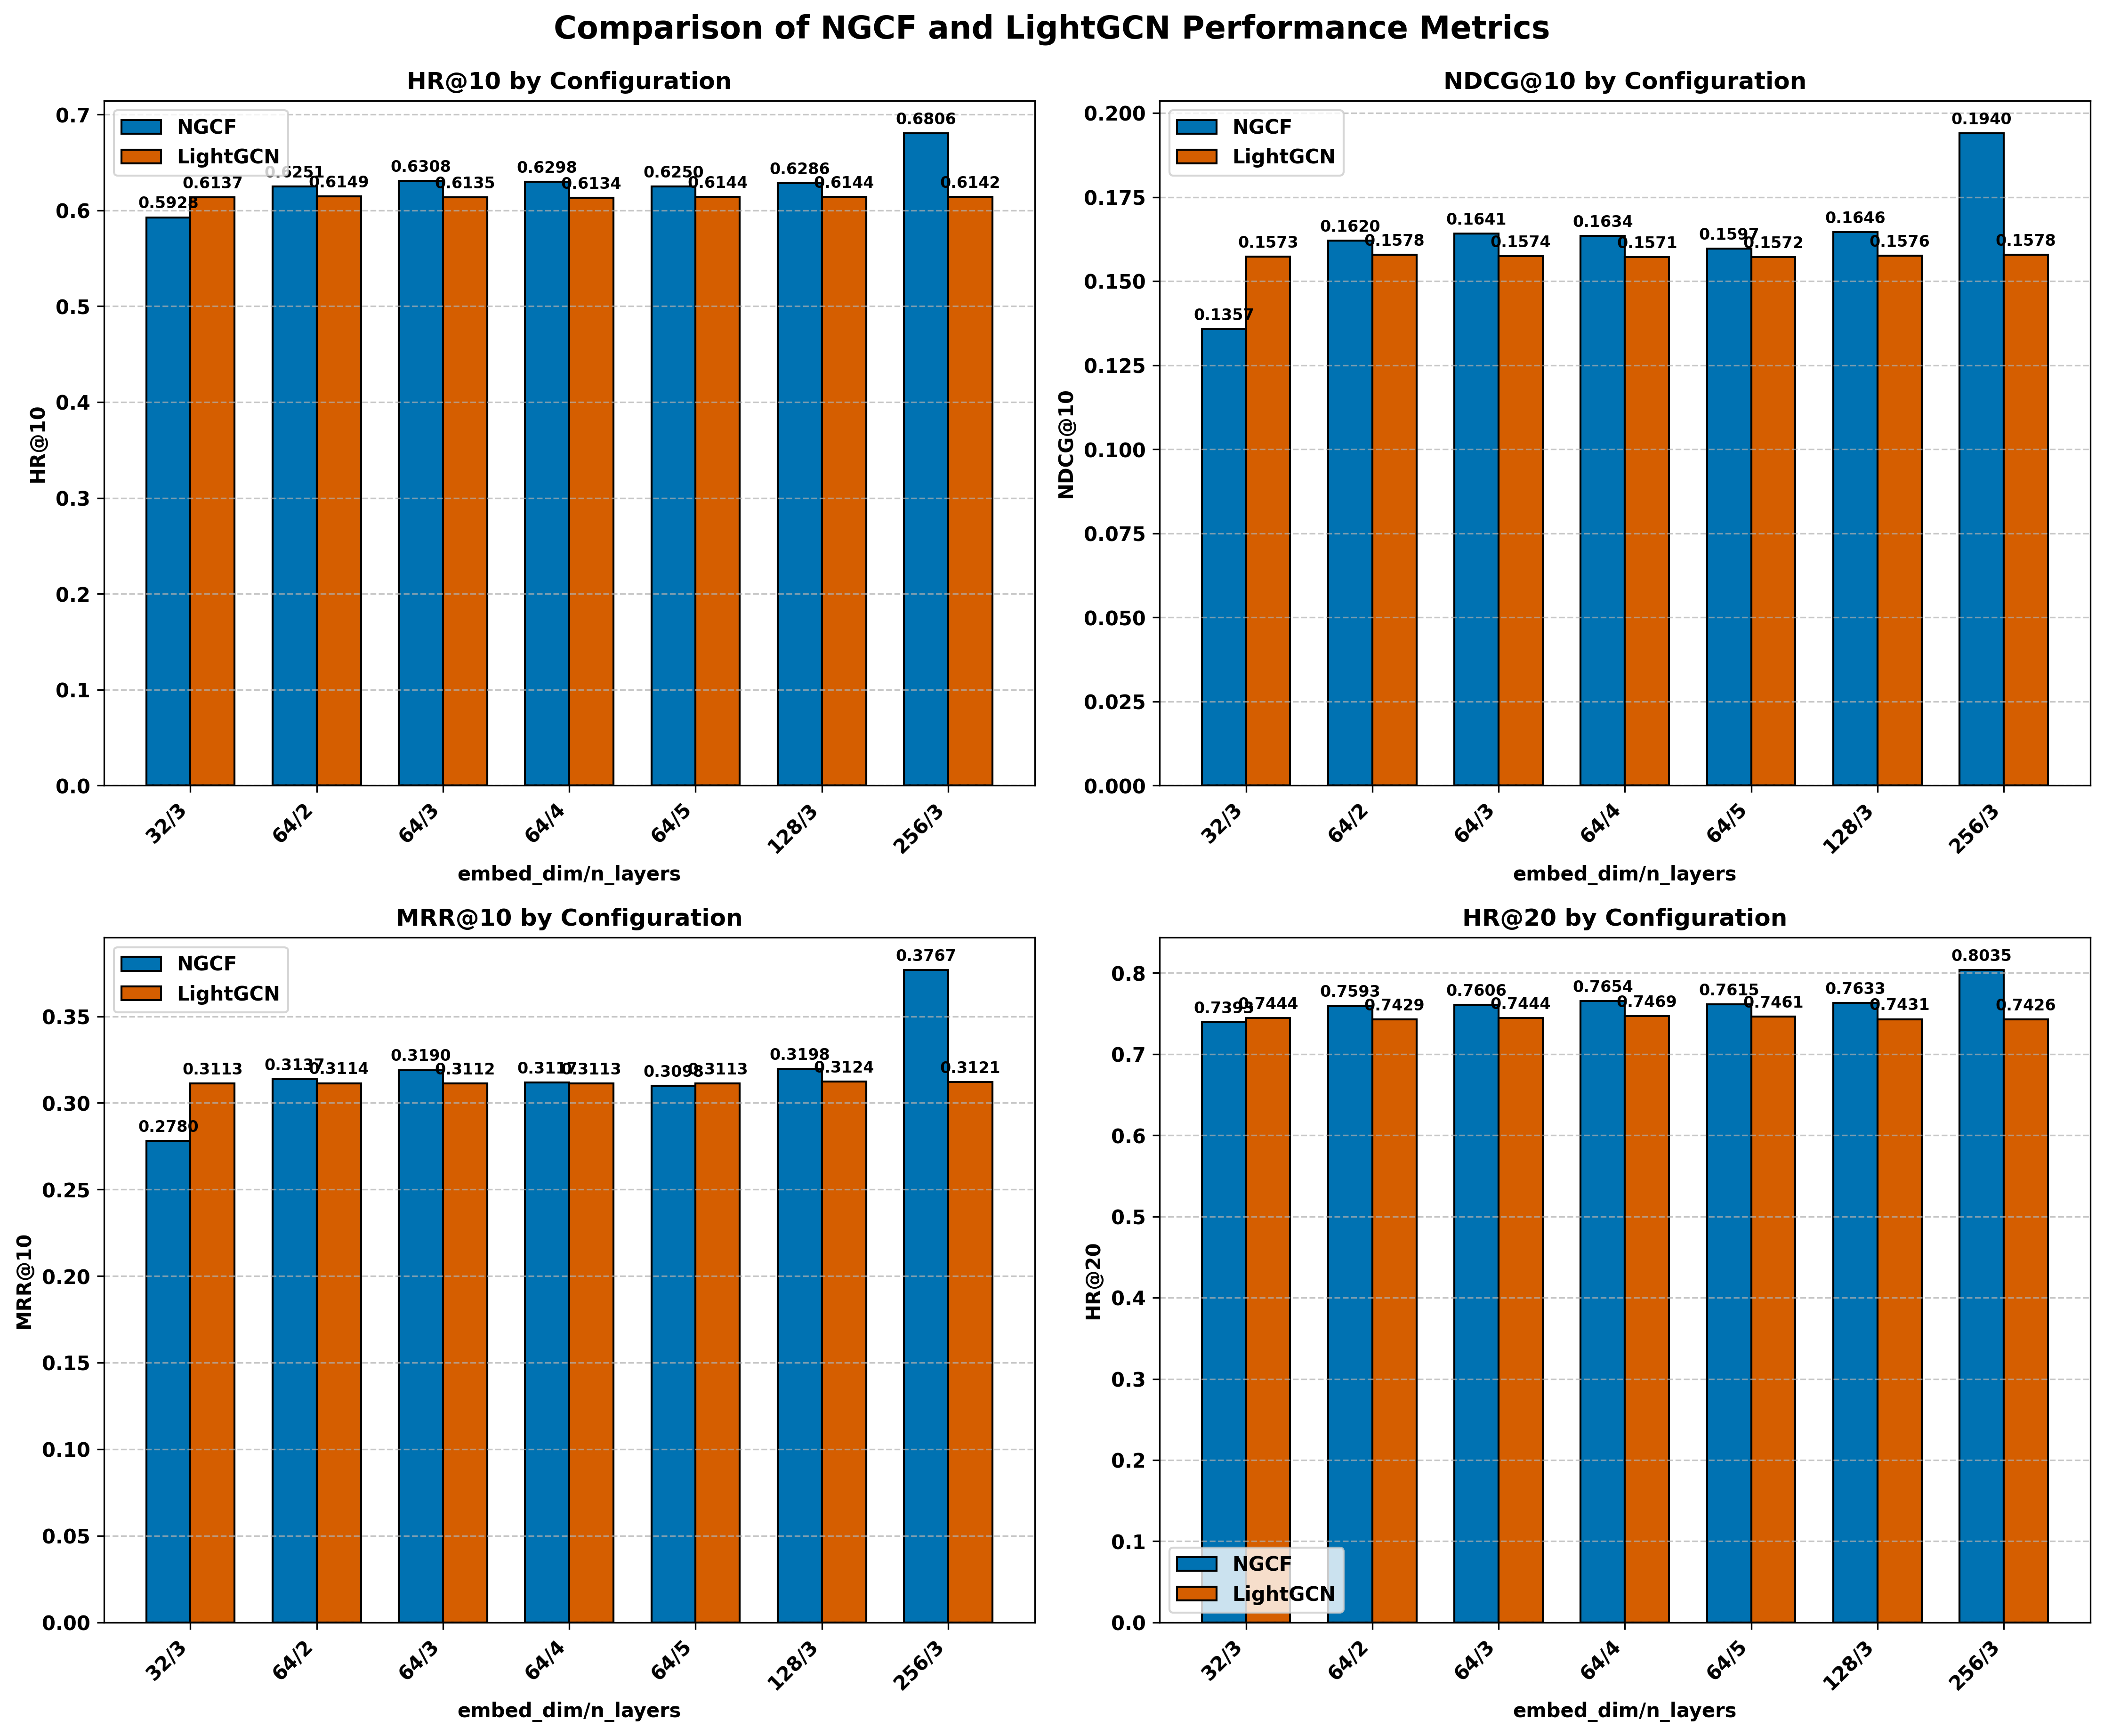
\includegraphics[width=\columnwidth]{model_comparison.png}  
\caption{Comparison of NGCF and LightGCN performance metrics across different embedding dimensions and layer configurations. The charts illustrate HR@10, NDCG@10, MRR@10, and HR@20 metrics, showing how both models respond to architecture variations.}  
\label{fig:model-comparison}  
\end{figure}  

For NGCF, we observed that increasing the embedding dimension significantly improves performance, with the best results achieved at embed\_dim=256 and n\_layers=3. This suggests that NGCF benefits from richer representation capacity to capture complex user-item interactions.  

Interestingly, LightGCN showed less sensitivity to hyperparameter variations, with relatively stable performance across different configurations. This aligns with the design philosophy behind LightGCN, which aimed to simplify the NGCF architecture by removing feature transformations and non-linearities.  

\section{Discussion and Implications}  

\subsection{Key Findings and Insights}  

Our experimental results yield several important insights:  

\begin{enumerate}  
    \item Traditional collaborative filtering methods remain highly competitive for recommendation tasks, particularly in domains with dense user-item interactions. However, this holds true for medium or small datasets; when dealing with very large datasets, the efficiency issues make it difficult for these algorithms to be applied directly in industrial settings. 
    
    \item The relative performance of algorithms varies significantly with dataset characteristics and evaluation protocols. No single algorithm consistently outperforms others across all settings.  
    
    \item Neural methods demonstrate advantages in temporal prediction scenarios, suggesting their ability to better capture evolving preference patterns.  
    
    \item The efficiency-effectiveness trade-off is an important consideration, with simpler methods like SVD offering substantial computational advantages with acceptable performance.  
    
    \item Hyperparameter tuning significantly impacts the performance of neural methods, with NGCF showing higher sensitivity compared to LightGCN.  
\end{enumerate}  

\subsection{Practical Recommendations}  

Based on our findings, we offer the following practical recommendations for recommendation system implementation:  

\begin{enumerate}  
    \item For small to medium-sized datasets with dense interactions, consider UserCF as a strong baseline that may outperform more complex approaches.  
    
    \item When computational efficiency is critical or for very large-scale applications, SVD and LightGCN offer good performance-efficiency trade-offs.  
    
    \item For applications where prediction of future interactions is important, neural methods like NGCF are preferred despite their higher computational requirements.  
    
    \item LightGCN is recommended over NGCF when computational resources are limited, as it offers comparable performance with fewer parameters and lower training time.  
    
    \item Careful hyperparameter tuning is essential for neural methods, particularly for NGCF where higher embedding dimensions can significantly improve performance.  
\end{enumerate}  

\subsection{Limitations and Future Work}  

While our study provides valuable insights, several limitations should be acknowledged:  

\begin{enumerate}  
    \item Our evaluation focused on two widely-used but moderately sized datasets. Future work should extend to larger-scale datasets with different sparsity characteristics.  
    
    \item We primarily evaluated general recommendation performance. Domain-specific requirements like diversity, novelty, or fairness were not considered.  
    
    \item Recent innovations in transformer-based recommendation algorithms were not included in our comparison.  
    
    \item Our evaluation metrics focused on ranking quality rather than other aspects like recommendation diversity or serendipity.  
\end{enumerate}  

Future research directions include investigating hybrid approaches that combine the strengths of traditional and neural methods, exploring the impact of different data augmentation techniques, and evaluating recommendation algorithms on multi-modal data incorporating textual, visual, and behavioral signals.  

  
\bibliographystyle{unsrt}   
\bibliography{references}  

\end{document} 
```

